\section{Evaluation}
\label{sec:evaluation}
We evaluate the performance of our solution on a single general purpose
Amazon EC2 m3.xlarge instance, running Debian 8.3 (Jessie)
and equipped with an Intel Xeon E5-2670 v2 (Ivy Bridge)  (2.6 GHz,
8 cores and 20 MB cache), 15 GB of RAM and a general purpose SSD.

The experimental framework consists in evaluating the timing and memory performance of Ontoqa when facing with questions caracterized by distinct sentence structures.

In particular we examine the following class of questions:

\begin{itemize}
	\item[Q1] questions in the form [pronoun,verb,object], e.g. \textit{who founded Microsoft?}.
	\item[Q2] questions in the form [pronoun,verb,relational noun,relational object], e.g. \textit{who are the corporate officers of Microsoft?}.
	\item[Q3] questions in the form [pronoun,copula,subject,verb], e.g. \textit{where is Microsoft headquartered?}.
	\item[Q4] questions in the form [pronoun,verb,superlative adjective,subject], e.g. \textit{which is the most valuable company?}.
	\item[Q5] questions in the form [copula,subject,adjective], e.g. \textit{is Satya Nadella italian?}.
	\item[Q6] questions in the form [copula,subject,verb,object,participle verb,object], e.g. \textit{did Microsoft acquire a company headquartered in Italy?}.
\end{itemize}

The reported results have been carried out by averaging measurements of 10 executions in random order. 
%
In Figure~\ref{fig:evaluation-time} and Figure~\ref{fig:evaluation-memory} we show, repsectively, the \textit{response time} and the \textit{memory usage} achieved by Ontoqa when facing the benchmark questions (Q1-6).
%
The former has been measured considering the time elapsed for the question to be answered, calling the Java built-in function \texttt{System.currentTimeMillis()}.
%
The latter has been measured considering the peak value of heap usage recorded by VisualVM.

\begin{figure}[tp]
	\centering
	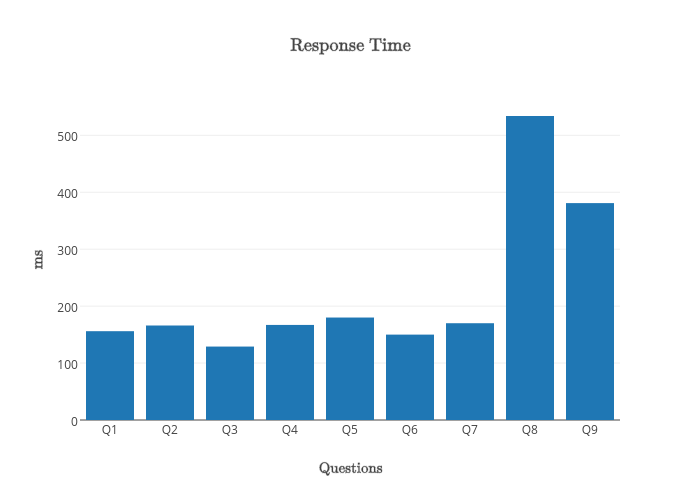
\includegraphics[width=0.8\columnwidth]{./fig/evaluation-response-time}
	\caption{Timing performance of Ontoqa facing the benchmark questions.}
	\label{fig:evaluation-time}
\end{figure}

\begin{figure}[tp]
	\centering
	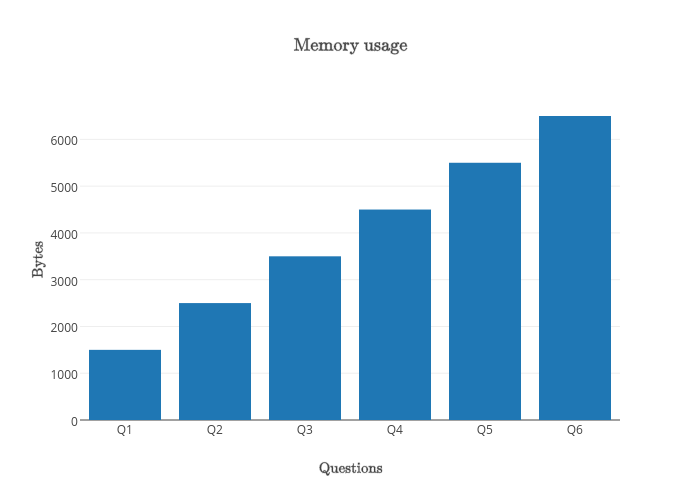
\includegraphics[width=0.8\columnwidth]{./fig/evaluation-memory-usage}
	\caption{Memory performance of Ontoqa facing the benchmark questions.}
	\label{fig:evaluation-memory}
\end{figure}